%
% assembly.tex
%
% Copyright (C) 2021 by SpaceLab.
%
% TTC Documentation
%
% This work is licensed under the Creative Commons Attribution-ShareAlike 4.0
% International License. To view a copy of this license,
% visit http://creativecommons.org/licenses/by-sa/4.0/.
%

%
% \brief Assembly instructions chapter.
%
% \author Gabriel Mariano Marcelino <gabriel.mm8@gmail.com>
%
% \institution Universidade Federal de Santa Catarina (UFSC)
%
% \version 1.2.0
%
% \date 2021/01/16
%

\chapter{Assembly Instructions} \label{ch:assembly}

This chapter will describe how to customize the radio configuration, power-on the board, import and flash the source code and finally alternatives to encode/decode to be transmitted/received packages from the TTC 2.0 module.

\section{Radio Configuration}\label{sec:wds}

This section is a tutorial designed to generate a source code file with basic configuration parameters for the radio module. To achieve this, the WDS software from Silicon Labs (version 3.2.11.0), which is only available on Windows, will be used.

\subsection{Steps}

After the installation of the software, the procedures to configure the beacon radio are described bellow.

\subsubsection{Step 1}

\begin{enumerate}
    \item Open the WDS software.
    \item The following box will appear in the center of the window.
    \item Click in "Simulate radio" and go to the next step.
\end{enumerate}

\begin{figure}[!h]
	\begin{center}
		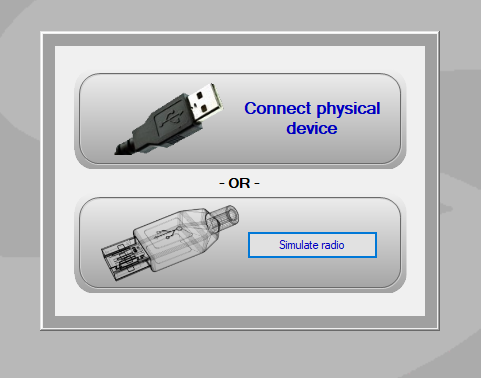
\includegraphics[width=0.5\textwidth]{figures/wds-tutorial/wds-tutorial-1.png}
		\caption{Step 1 of the radio configuration.}
		\label{fig:wds-tutorial-step-1}
	\end{center}
\end{figure}

\subsubsection{Step 2}

\begin{enumerate}
    \item In the list of radios that appeared on the new window, select the chip type ``Si4463".
    \item In the revision column, select ``B1".
    \item Click on ``Select Radio" to go to the next step.
\end{enumerate}

\begin{figure}[!h]
	\begin{center}
		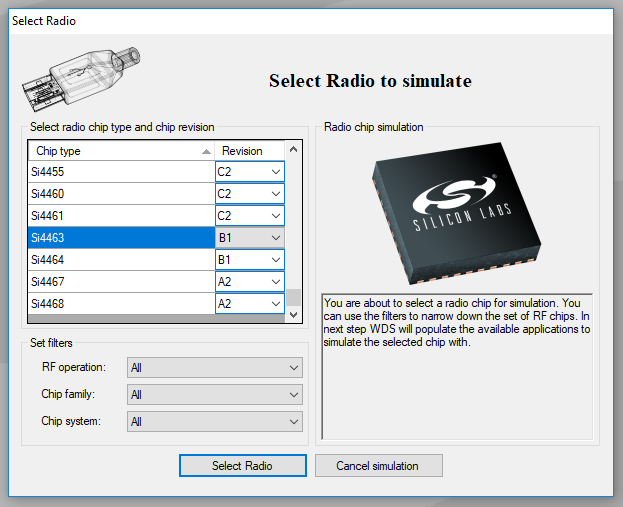
\includegraphics[width=0.75\textwidth]{figures/wds-tutorial/wds-tutorial-2.png}
		\caption{Step 2 of the radio configuration.}
		\label{fig:wds-tutorial-step-2}
	\end{center}
\end{figure}

\subsubsection{Step 3}

\begin{enumerate}
    \item Select ``Radio Configuration Application".
    \item Click on ``Select Application" to go to the next step.
\end{enumerate}

\begin{figure}[!h]
	\begin{center}
		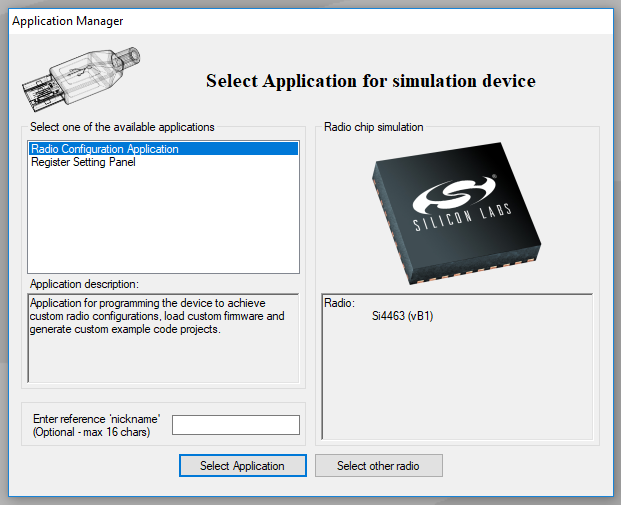
\includegraphics[width=0.75\textwidth]{figures/wds-tutorial/wds-tutorial-3.png}
		\caption{Step 3 of the radio configuration.}
		\label{fig:wds-tutorial-step-3}
	\end{center}
\end{figure}

\subsubsection{Step 4}

\begin{enumerate}
    \item In the ``Frequency and power" tab, change the base frequency to 145,9 MHz.
    \item Change the channel spacing to 0 kHz.
    \item Change the crystal tolerance to 10,0 ppm (Both RX and TX).
    \item Go to the next step.
\end{enumerate}

\begin{figure}[!h]
	\begin{center}
		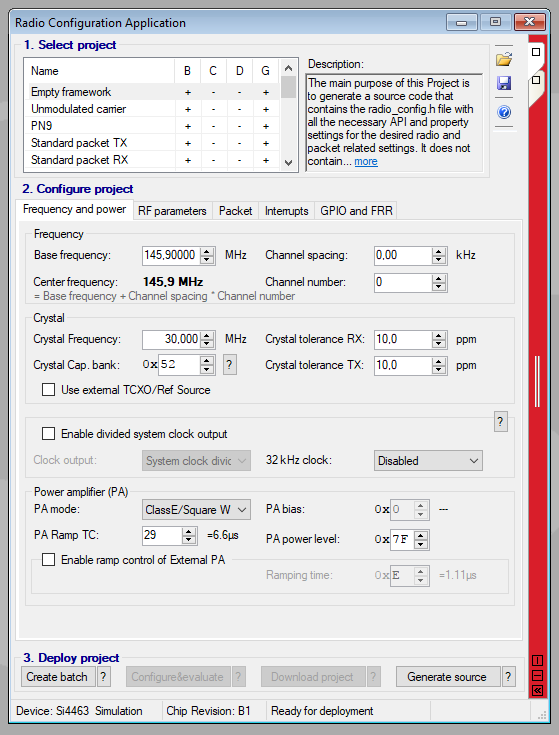
\includegraphics[width=0.75\textwidth]{figures/wds-tutorial/wds-tutorial-4.png}
		\caption{Step 4 of the radio configuration.}
		\label{fig:wds-tutorial-step-4}
	\end{center}
\end{figure}

\subsubsection{Step 5}

\begin{enumerate}
    \item In the ``RF parameters" tab, change the modulation type to ``2GFSK".
    \item Change the the data rate to 1,2 kbps.
    \item Change the deviation to $2,5\ kHz$.
    \item Go to the next step.
\end{enumerate}

\begin{figure}[!h]
	\begin{center}
		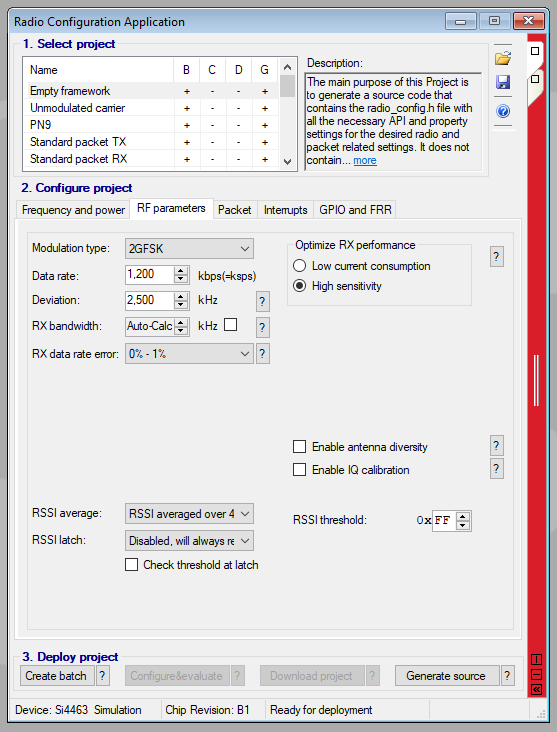
\includegraphics[width=0.75\textwidth]{figures/wds-tutorial/wds-tutorial-5.png}
		\caption{Step 5 of the radio configuration.}
		\label{fig:wds-tutorial-step-5}
	\end{center}
\end{figure}

\subsubsection{Step 6}

\begin{enumerate}
    \item In the ``Packet" tab, many subtabs will appear. In ``Preamble" change the ``Preamble TX length" to 4 bytes.
    \item Again, in ``Preamble", change the ``Preamble pattern" to ``Std. 1010 pattern (>= 32 and < 40 bits)".
    \item Go to the next step.
\end{enumerate}

\begin{figure}[!h]
	\begin{center}
		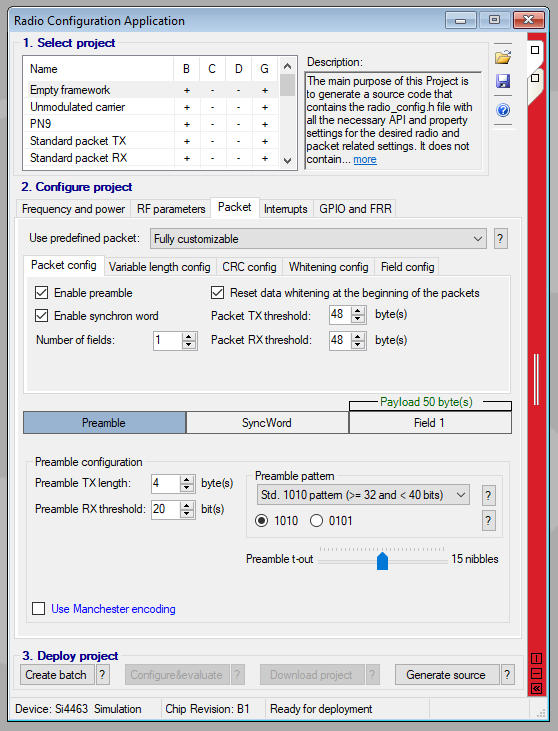
\includegraphics[width=0.75\textwidth]{figures/wds-tutorial/wds-tutorial-6.png}
		\caption{Step 6 of the radio configuration.}
		\label{fig:wds-tutorial-step-6}
	\end{center}
\end{figure}

\subsubsection{Step 7}

\begin{enumerate}
    \item In the ``Sync Word" tab, change the sync word length field to ``4 bytes".
    \item In the ``Sync Word (on air int.)", enter the following sequence: 5D E6 2A 7E. This sequence is the sync word used by the NGHam protocol.
    \item Go to the next step.
\end{enumerate}

\begin{figure}[!h]
	\begin{center}
		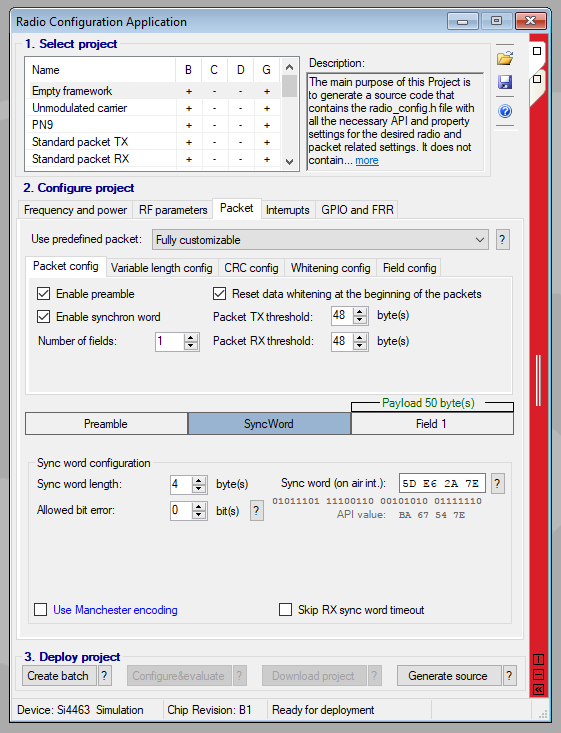
\includegraphics[width=0.75\textwidth]{figures/wds-tutorial/wds-tutorial-7.png}
		\caption{Step 7 of the radio configuration.}
		\label{fig:wds-tutorial-step-7}
	\end{center}
\end{figure}

\subsubsection{Step 8}

\begin{enumerate}
    \item In the ``Field 1" tab, change the ``Field length" to 50 bytes.
    \item Go to the next step.
\end{enumerate}

\begin{figure}[!h]
	\begin{center}
		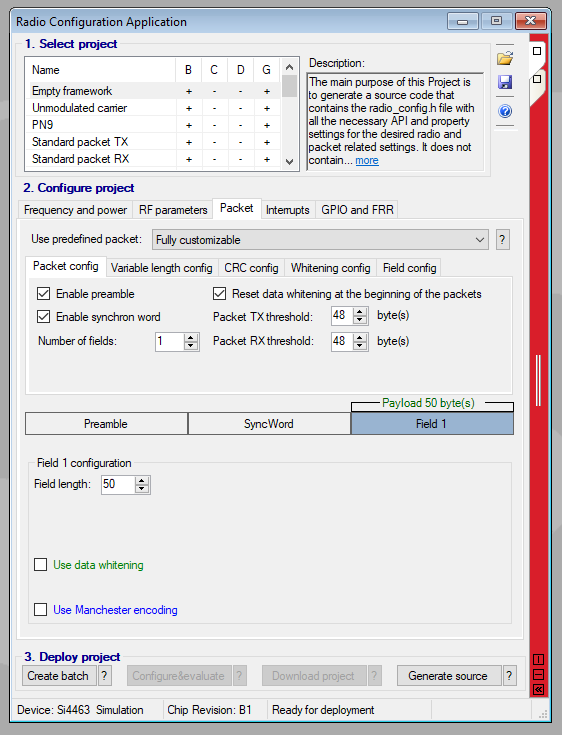
\includegraphics[width=0.75\textwidth]{figures/wds-tutorial/wds-tutorial-8.png}
		\caption{Step 8 of the radio configuration.}
		\label{fig:wds-tutorial-step-8}
	\end{center}
\end{figure}

\subsubsection{Step 9}

\begin{enumerate}
    \item In the ``Variable length config" tab, there is no values to change.
    \item Go to the next step.
\end{enumerate}

\begin{figure}[!h]
	\begin{center}
		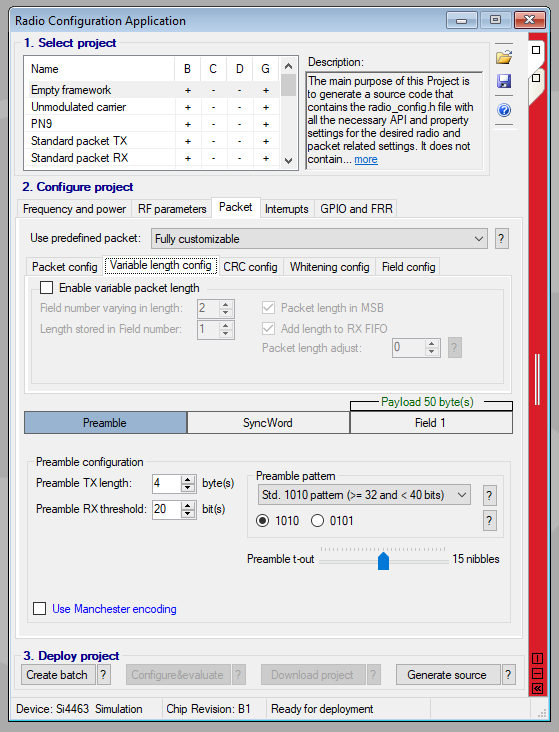
\includegraphics[width=0.75\textwidth]{figures/wds-tutorial/wds-tutorial-9.png}
		\caption{Step 9 of the radio configuration.}
		\label{fig:wds-tutorial-step-9}
	\end{center}
\end{figure}

\subsubsection{Step 10}

\begin{enumerate}
    \item In the ``CRC config" tab, choose ``No CRC." in ``CRC polynomial".
    \item Go to the next step.
\end{enumerate}

\begin{figure}[!h]
	\begin{center}
		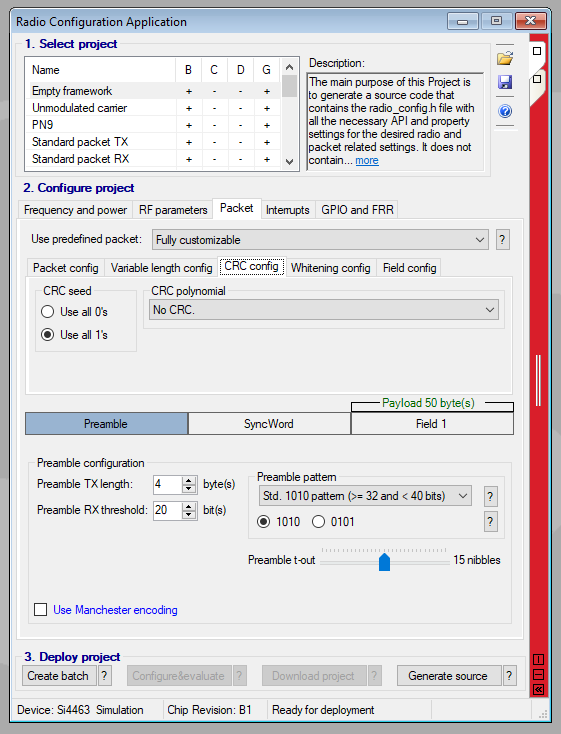
\includegraphics[width=0.75\textwidth]{figures/wds-tutorial/wds-tutorial-10.png}
		\caption{Step 10 of the radio configuration.}
		\label{fig:wds-tutorial-step-10}
	\end{center}
\end{figure}

\subsubsection{Step 11}

\begin{enumerate}
    \item In the ``Whitening config" tab, there is no values to change.
    \item Go to the next step.
\end{enumerate}

\begin{figure}[!h]
	\begin{center}
		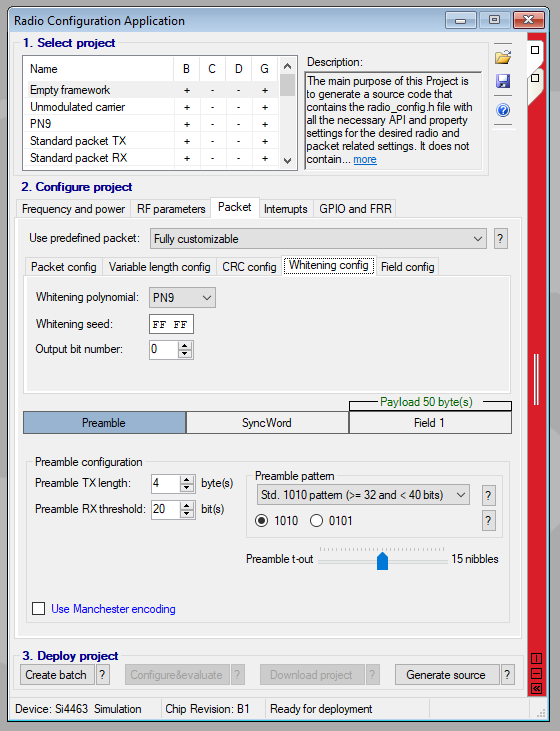
\includegraphics[width=0.75\textwidth]{figures/wds-tutorial/wds-tutorial-11.png}
		\caption{Step 11 of the radio configuration.}
		\label{fig:wds-tutorial-step-11}
	\end{center}
\end{figure}

\subsubsection{Step 12}

\begin{enumerate}
    \item In the ``Field config" tab, there is no values to change.
    \item Go to the next step.
\end{enumerate}

\begin{figure}[!h]
	\begin{center}
		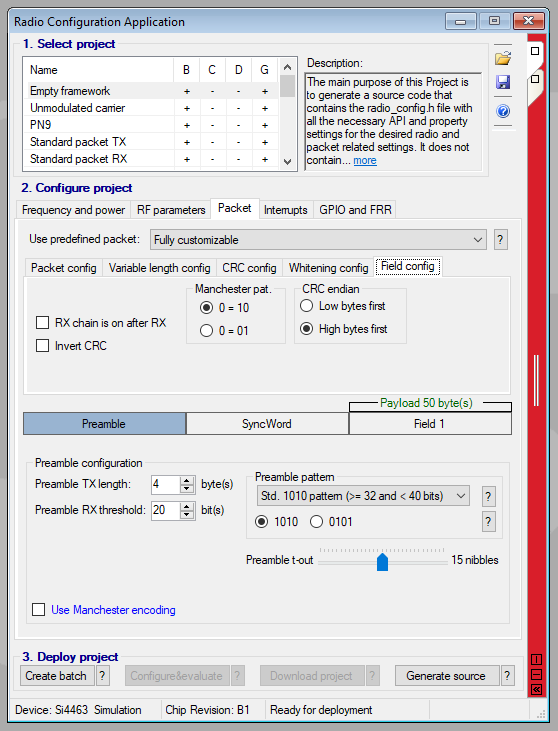
\includegraphics[width=0.75\textwidth]{figures/wds-tutorial/wds-tutorial-12.png}
		\caption{Step 12 of the radio configuration.}
		\label{fig:wds-tutorial-step-12}
	\end{center}
\end{figure}

\subsubsection{Step 13}

\begin{enumerate}
    \item In the ``Interrupts" tab, there is no values to change.
    \item Go to the next step.
\end{enumerate}

\begin{figure}[!h]
	\begin{center}
		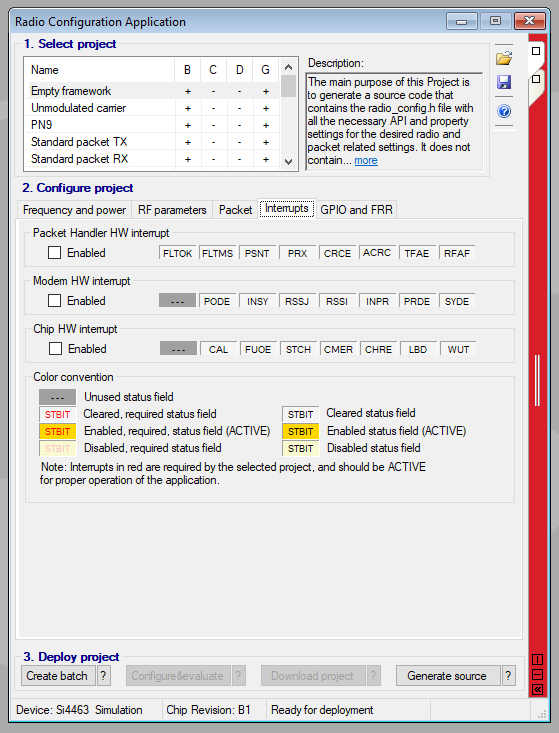
\includegraphics[width=0.75\textwidth]{figures/wds-tutorial/wds-tutorial-13.png}
		\caption{Step 13 of the radio configuration.}
		\label{fig:wds-tutorial-step-13}
	\end{center}
\end{figure}

\subsubsection{Step 14}

\begin{enumerate}
    \item In the ``GPIO and FRR" tab, enable pullup in GPIO1 and choose ``TX\_FIFO\_EMPTY - This output is..." as functionality.
    \item Enable pullup in GPIO2 and choose ``RX\_STATE - This output is..." as functionality.
    \item Enable pullup in GPIO3 and choose ``TX\_STATE - This output is..." as functionality.
    \item Enable pullup in NIRQ and choose ``Active low interrupt signal" as functionality.
    \item Enable pullup in SDO and choose ``SDO - Output SPI Serial data out." as functionality.
    \item Select ``Global status" for the ``Fast Response Register A".
    \item Select ``Global interrupt pending" for the ``Fast Response Register B".
    \item Select ``Packet Handler status" for the ``Fast Response Register C".
    \item Select ``Chip status" for the ``Fast Response Register D".
    \item Go to the next step.
\end{enumerate}

\begin{figure}[!h]
	\begin{center}
		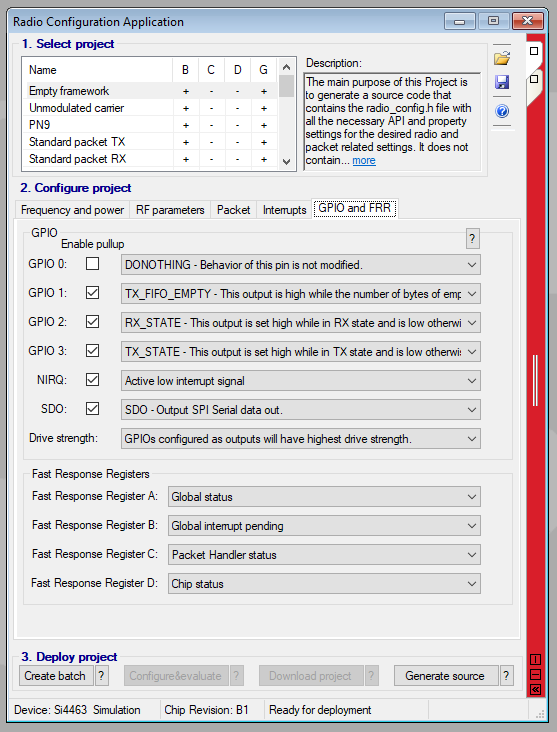
\includegraphics[width=0.75\textwidth]{figures/wds-tutorial/wds-tutorial-14.png}
		\caption{Step 14 of the radio configuration.}
		\label{fig:wds-tutorial-step-14}
	\end{center}
\end{figure}

\subsubsection{Step 15}

\begin{enumerate}
    \item Click in ``Generate Source" and select the ``.h" type of source.
    \item The software will ask where to save the generated file.
    \item The generated *.h file must be copied to the directory of the rf4463 driver.
\end{enumerate}

\subsection{Final Remarks}

This tutorial has the objective of generate a basic configuration parameters of the radio, some functionalities of the radio are not covered by the WDS software, and so, must be configured/controlled in the device driver.

\section{Powering the module}

The TTC 2.0 has three power supply inputs: one 3V3 supply to power the MCU and all the external components, two 5V inputs to power the transceivers.

The 3V3 input voltage rail is accessible at the PC-104 H2-27 and H2-28 pins. You can also supply the 3V3 rail with MSP-FET JTAG connector by connecting the jumper CN9. This last option should only be used for debug as it requires the MSP-430 FET to be connected.

The transceiver supply rails are only accessible on the PC-104: H1-49 and H1-50 for radio 0 and H1-51 and H1-52 for radio 1. 

The TTC 2.0 module has only one common ground and it can be accessed by multiple pins on the PC-104 (see \autoref {tab:pc104-signals})

It is recommended, for safety reasons, to use different supply channels for each supply rail. Also, for extra safety it is recommended to add current cut-off limits: use $30 mA$ for the 3V3 and $500 mA$ for the radio 5V power rails. 

\section{Compiling, Building and Flashing the source code}

This tutorial is a reference to compile, build and flash the firmware of the TTC 2.0 module using the Texas Instruments IDE: Code Composer Studio (CCS) version 12.

%All the software development was made using the Code Composer Studio (CCS) IDE, version 12. To load the code into the TTC 2.0 MCU, the MSP-FET can be used.

\subsection{Importing the Source Code in the CCS IDE}
The TTC 2.0 releases are available to download at the TTC 2.0 Github releases page \cite{ttc2-releases}. The CCS IDE is available at the Texas Instruments website \cite{ccs-studio}.

The steps bellow describe how to import the source code in the CCS IDE:

\begin{enumerate}
    \item Extract the ttc2-x.x.zip file.  
    \item Open the CCS IDE.
    \item Go to ``Project" -> ``Import CCS Projects...".
    \item The window from the figure \ref{fig:compiling-tutorial} will appear on the screen.
    \item On ``Select search-directory:" select ``\textit{project\_path/ttc2-x.x/firmware}".
    \item Click on ``Finish".
    
    \item After importing the project, select the project on the ``Project Explorer" and open the ``Properties" tab (you can use the shortcut \textit{Alt+Enter} or right-click on the project's name). 
    \item The window from the figure \ref{fig:project_properties} will appear on the screen.
    \item On ``Variant", select the MCU partnumber (MSP430F6659 or MSP430F5659).
    \item On ``Compiler Version", select ``TI v21.6.1.LTS`` or higher.
    \item Click on ``Apply and Close".
\end{enumerate}

\begin{figure}[!h]
	\begin{center}
		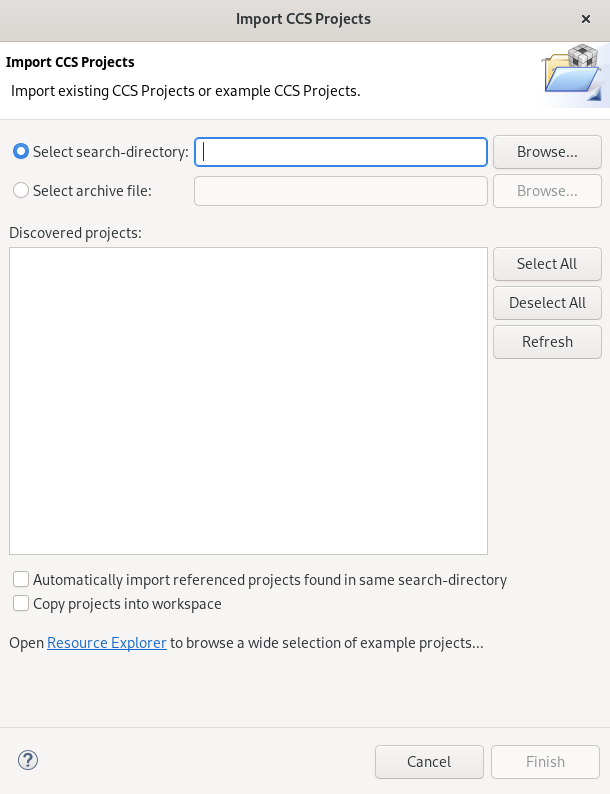
\includegraphics[width=0.75\textwidth]{figures/ccs_project.png}
		\caption{New CCS project window.}
		\label{fig:compiling-tutorial}
	\end{center}
\end{figure}

\begin{figure}[!h]
	\begin{center}
		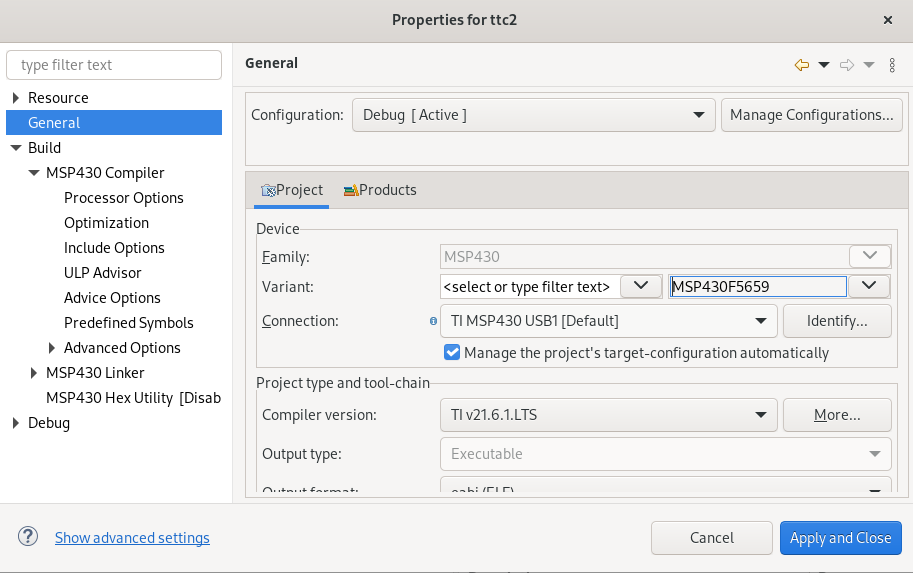
\includegraphics[width=0.75\textwidth]{figures/ccs_properties.png}
		\caption{CCS project's properties window.}
		\label{fig:project_properties}
	\end{center}
\end{figure}

\subsection{Customize the project}
Since the TTC 2.0 has two MCU modules it is needed to specific which one you want to target. Access the configuration header file on the ``Project Explorer" at ``\textit{config/config.h}", change the ``RADIO\_MODULE" macro between '0' or '1' (The module '1' is the one closest to the PC-104).

Each MCU module controls a corresponding transceiver, to customize the transceiver configuration (as shown on section \ref{sec:wds}) copy all the code on the header file generated by the WDS software and paste it at the ``config/radio\_x\_config.h".

\subsection{Compiling and Building}
To compile and build the firmware, click on "Project" -> "Build Project".

\subsection{Flashing}

With the board turned on and the MSP-FET connected, click on ``Run" -> ``Load". If no errors occur, the firmware was loaded successfully to the board.

\section{Receiving and sending Telecommands}

The structure of the telecommands are described at \autoref{ch:operation}. The standard solution to implement a ground-station is using the SpaceLab transmitter and decoder solutions \cite{sl-transmitter} \cite{sl-decoder} combined with and RTL-SDR.
